\begin{frame}{Bonnes pratiques dans le numérique}{Conseil 22/115}

\begin{block}{Écrire des sélecteurs CSS efficaces}
Privilégier les sélecteurs basés sur des ID ou des classes. Ils seront ainsi filtrés plus rapidement, économisant des cycles CPU à la machine interprétant les règles.
 \end{block}

\begin{minipage}[b]{0.7\linewidth}
\begin{alertblock}{Ne pas écrire}
\begin{figure}
    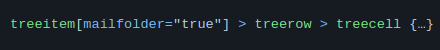
\includegraphics[scale=0.4]{chapitre2/wdd3/fig/c1.png}
    \centering
\end{figure}
 \end{alertblock}
\end{minipage}\hfill
\begin{minipage}[b]{0.3\linewidth}
\begin{exampleblock}{Mais plutôt}
\begin{figure}
    
\includegraphics[scale=0.4]{chapitre2/wdd3/fig/c2.png}
    \centering
\end{figure}
 \end{exampleblock}
\end{minipage}\hfill

\begin{minipage}[b]{0.7\linewidth}
\begin{alertblock}{Ne pas écrire}
\begin{figure}
    
\includegraphics[scale=0.5]{chapitre2/wdd3/fig/c3.png}
    \centering
\end{figure}
 \end{alertblock}
\end{minipage}\hfill
\begin{minipage}[b]{0.3\linewidth}
\begin{exampleblock}{Mais plutôt}
\begin{figure}
    
\includegraphics[scale=0.4]{chapitre2/wdd3/fig/c4.png}
    \centering
\end{figure}
 \end{exampleblock}
\end{minipage}\hfill


\end{frame}


\begin{frame}{Bonnes pratiques dans le numérique}{Conseils 24-26/115}
\begin{block}{Grouper les déclarations CSS similaires}
Lorsque plusieurs éléments du DOM (Document Object Model) ont des propriétés CSS communes, les déclarer ensemble dans la même feuille de styles. Cette méthode permet de réduire le poids de la CSS.
\end{block}

\begin{block}{Utiliser les notations CSS abrégées}
\begin{minipage}[b]{0.7\linewidth}
\begin{alertblock}{Ne pas écrire}
\begin{figure}
    
\includegraphics[scale=0.35]{chapitre2/wdd3/fig/c5.png}
    \centering
\end{figure}
 \end{alertblock}
\end{minipage}\hfill
\begin{minipage}[b]{0.3\linewidth}
\begin{exampleblock}{Mais plutôt}
\begin{figure}
    
\includegraphics[scale=0.49]{chapitre2/wdd3/fig/c6.png}
    \centering
\end{figure}
 \end{exampleblock}
\end{minipage}\hfill

\end{block}


\begin{block}{Fournir une CSS print}
La feuille de styles réduit le nombre de pages imprimées, et donc indirectement l’empreinte écologique du site web (dépouillée, police de caractères économe en encre.

\end{block}

\end{frame}


\begin{frame}{Bonnes pratiques dans le numérique}{Conseils 27-29/115}

\begin{block}{Favoriser les polices standards}
Elles sont déjà présentes sur l’ordinateur de l’utilisateur (absence de téléchargement). 
\end{block}

\begin{block}{Préférer les glyphs aux images}
\begin{itemize}
    \item Réduire la bande passante en économisant sur le poids
    \item Réduire le nombre de requêtes
    \item Réduire la complexité du DOM, notamment avec de nombreux pictogrammes SVG
\end{itemize}
\end{block}

\begin{block}{Valider les pages auprès du W3C}
Utiliser le validateur du W3C (World Wide Web Consortium) pour vérifier que les pages sont bien valides et que le code HTML est correctement formé : https://validator.w3.org
\end{block}

\end{frame}



\begin{frame}{Externaliser les CSS et JavaScript}{Conseils 30-32/115}

\begin{block}{Externaliser les CSS et JavaScript}
Veiller à ce que les codes CSS et JavaScript ne soient pas embarqués dans le code HTML de la page, à l’exception d’éventuelles variables de configuration pour les objets JavaScript.


\begin{minipage}[b]{0.5\linewidth}
\begin{alertblock}{Ne pas écrire}
\begin{figure}
    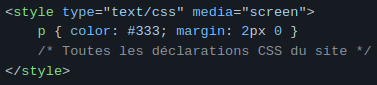
\includegraphics[scale=0.4]{chapitre2/wdd3/fig/c7.png}
    \centering
\end{figure}
 \end{alertblock}
\end{minipage}\hfill
\begin{minipage}[b]{0.45\linewidth}
\begin{exampleblock}{Mais plutôt}
\begin{figure}
    
\includegraphics[scale=0.35]{chapitre2/wdd3/fig/c8.png}
    \centering
\end{figure}
 \end{exampleblock}
\end{minipage}\hfill

\end{block}

\begin{block}{Ne pas redimensionner les images coté navigateur}
Générer les images à la taille à laquelle elles sont affichées.
\end{block}


\begin{block}{Eviter d'utiliser des images matricielles pour l'interface}
Privilégier l'approche vectorielle.
\end{block}


\end{frame}






\begin{frame}{Pause débunkage }{Le greenWashing}
\begin{figure}
    \centering
    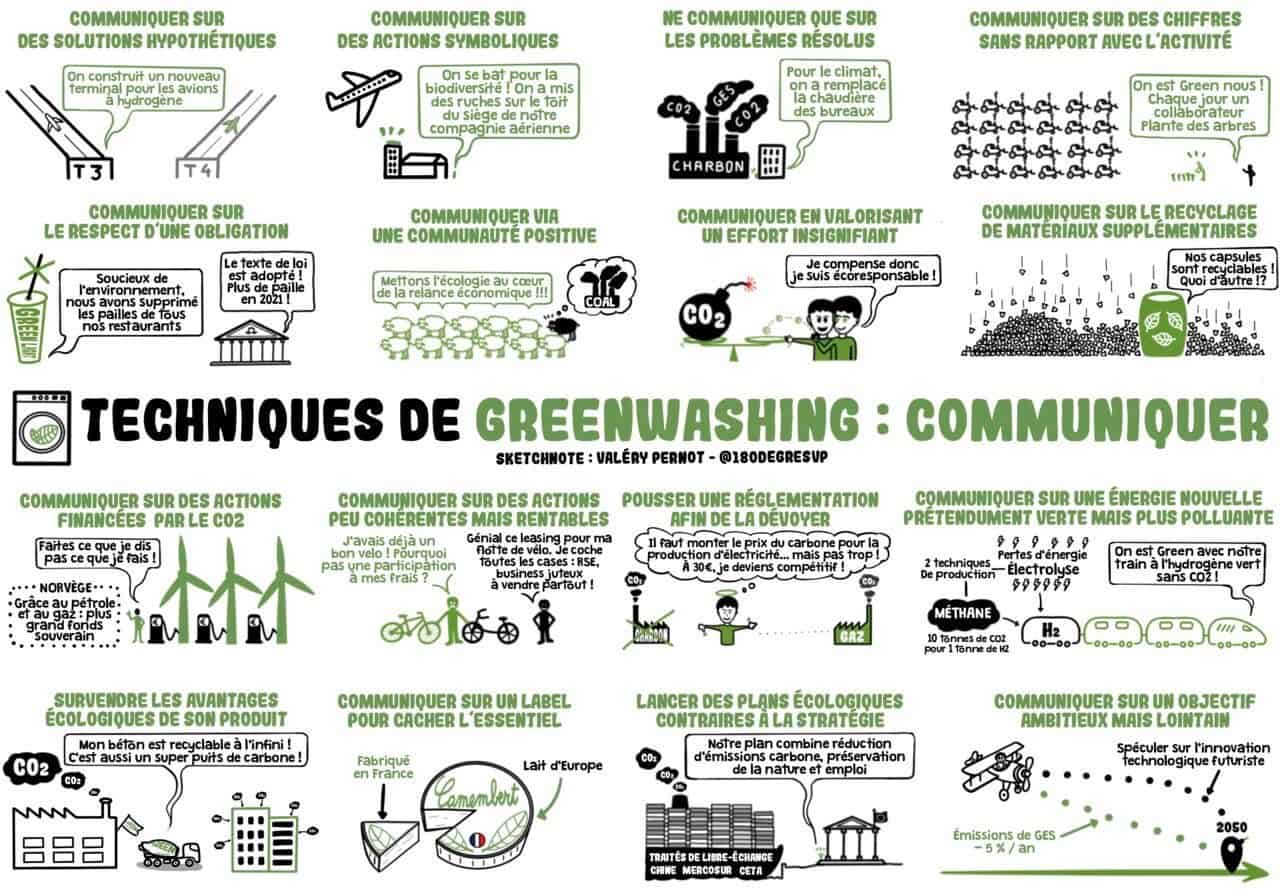
\includegraphics[scale=0.235]{chapitre2/wdd3/fig/greenwashing.jpg}
\end{figure}
\end{frame}